\documentclass[11pt, a4paper, twocolumn]{article}
\usepackage[utf8]{inputenc}
\usepackage{graphicx}
\usepackage{listings}
\usepackage{bookmark}
\PassOptionsToPackage{hyphens}{url}\usepackage{hyperref}
\usepackage{amsmath,amsfonts,amssymb}
\usepackage{geometry}
 \geometry{
 left=20mm,
 right=20mm,
 top=20mm,
 bottom=20mm
 }

\graphicspath{ {./plots/} }

\begin{document}
\date{2019 December}
\title{CS-443 Machine Learning Project 2: TwitterOnFire}
\author{
  Julie Camille Rosalie Giunta\\
  \texttt{274957}
  \and
  Samuel Chassot\\
  \texttt{270955}
  \and
  Daniel Filipe Nunes Silva\\
  \texttt{275197}
}

\maketitle
\clearpage

\section{Introduction}
In this project, we implement tweets classifiers using logistic regression, support-vector machine, neural nets and BERT to predict if their content is positive or negative.

\section{Logistic Regression and Support-Vector Machine}
In this section, we assess basic machine learning techniques. First, we present the preprocessing steps we applied to clean, normalize and transform the provided tweets datasets. Then, we compare them by training two models using support-vector machine and logistic regression classifiers. Finally, we optimize the most accurate models.

We used the following libraries and their dependencies.
\begin{itemize}
	\setlength\itemsep{1px}
	\item Python 3.8
	\item Jupyter-Notebook
	\item Natural Language Toolkit
	\item Scikit-learn
\end{itemize}

\subsection{Preprocessing}
We applied three kinds of preprocessing steps.
\begin{itemize}
	\setlength\itemsep{1px}
	\item Removing or replacing words and symbols.
	\item Normalizing by modifying words or sentences.
	\item Transforming the tweets into usable data structures for machine learning.
\end{itemize}

\subsubsection{Tweet Cleaning}
This is a basic operation. We get rid of \texttt{<User>}, \texttt{<url>} and \verb"\n" because these have already been processed and should not contain that much information. Notice that nice users and bad users are all described by the same word. The same argument can be applied to URLs. We also use regular expression to remove all kinds of punctuation. Even if punctation is usually expressive, it may be inconsistent considering the variety of tweets.

\subsubsection{Duplicates}
We simply remove all the duplicates tweets in the cleaned datasets. The problem with duplicates is that they can artificially increase the accuracy if the sames tweets appear in the training as well as in the test dataset. Nevertheless, removing duplicates do not necessarly make sense as multiple user could have written the same tweet. We would neglect its importance.

\subsubsection{Stemming}
Stemming is a technique that removes affixes so that similar words are effectively understood as similar when interpreted by the machine learning algorithm. Here are some examples : \textit{cars - car, swimming - swimm, this - thi}. This is often described as brute force as it is not smart but crude. For example, it does not see the difference between a word in its plural form from a word whose last letter is an \textit{s}.

\subsubsection{Lemmatization}
This technique is the smart version of stemming. It does a more advanced analysis of word to clearly identify the structure of each word and to cut it correctly.

\subsubsection{Stop Words}
Stop words are the most common words like \textit{I, it, is, of, in, \dots}. They should be equivalently be present in both positive and negative datasets but they do not have real impact in the meaning of the sentence. We went trough all the datasets to establish a list of the most used words, kept the ten most used and removed them in all the tweets of the training sets.

\subsubsection{Vectorization}
We use Scikit-learn to vectorize our data. We used multiple binary vectorization with \textit{n-grams} where \textit{n} corresponds to the number of words vectorized together. This helps considering the context in which words are used by increasing \textit{n}.

\subsubsection{Term Frequency-Inverse Document Frequency}
Instead of using \textit{0s} and \textit{1s} like binary vectorization, with \textit{TF-IDF} we count the occurences of the words.

\subsection{1-grams Logistic Regression and Support-Vector Machine}
First, we select the most effective cleaning or normalizing method by assessing them with logistic regression and SVM on a 1-grams vectorization. We use 75\% of the provided datasets for the training and the 25\% remaining for testing.

\begin{figure}[h]
	\centering
	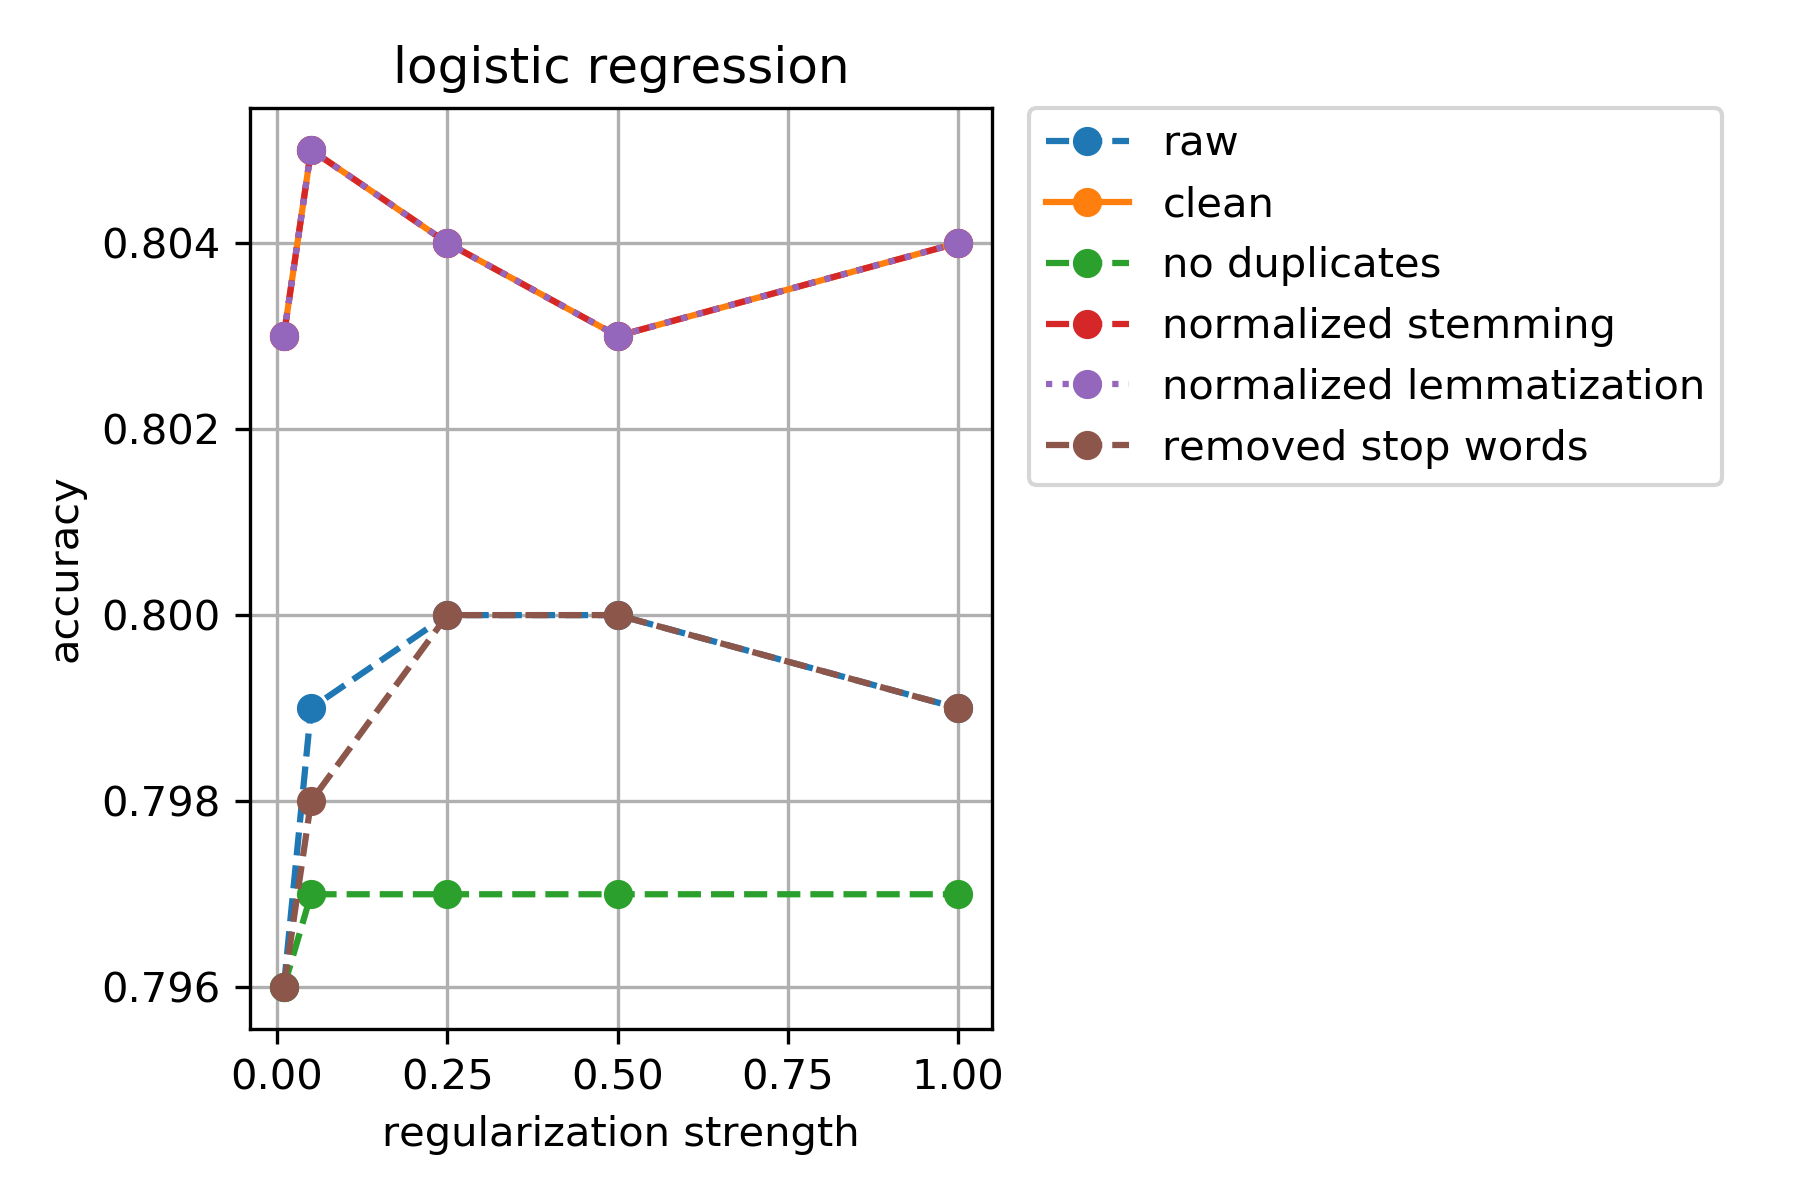
\includegraphics[width=0.5\textwidth]{../plots/logreg.png}
\end{figure}

\begin{figure}[h]
	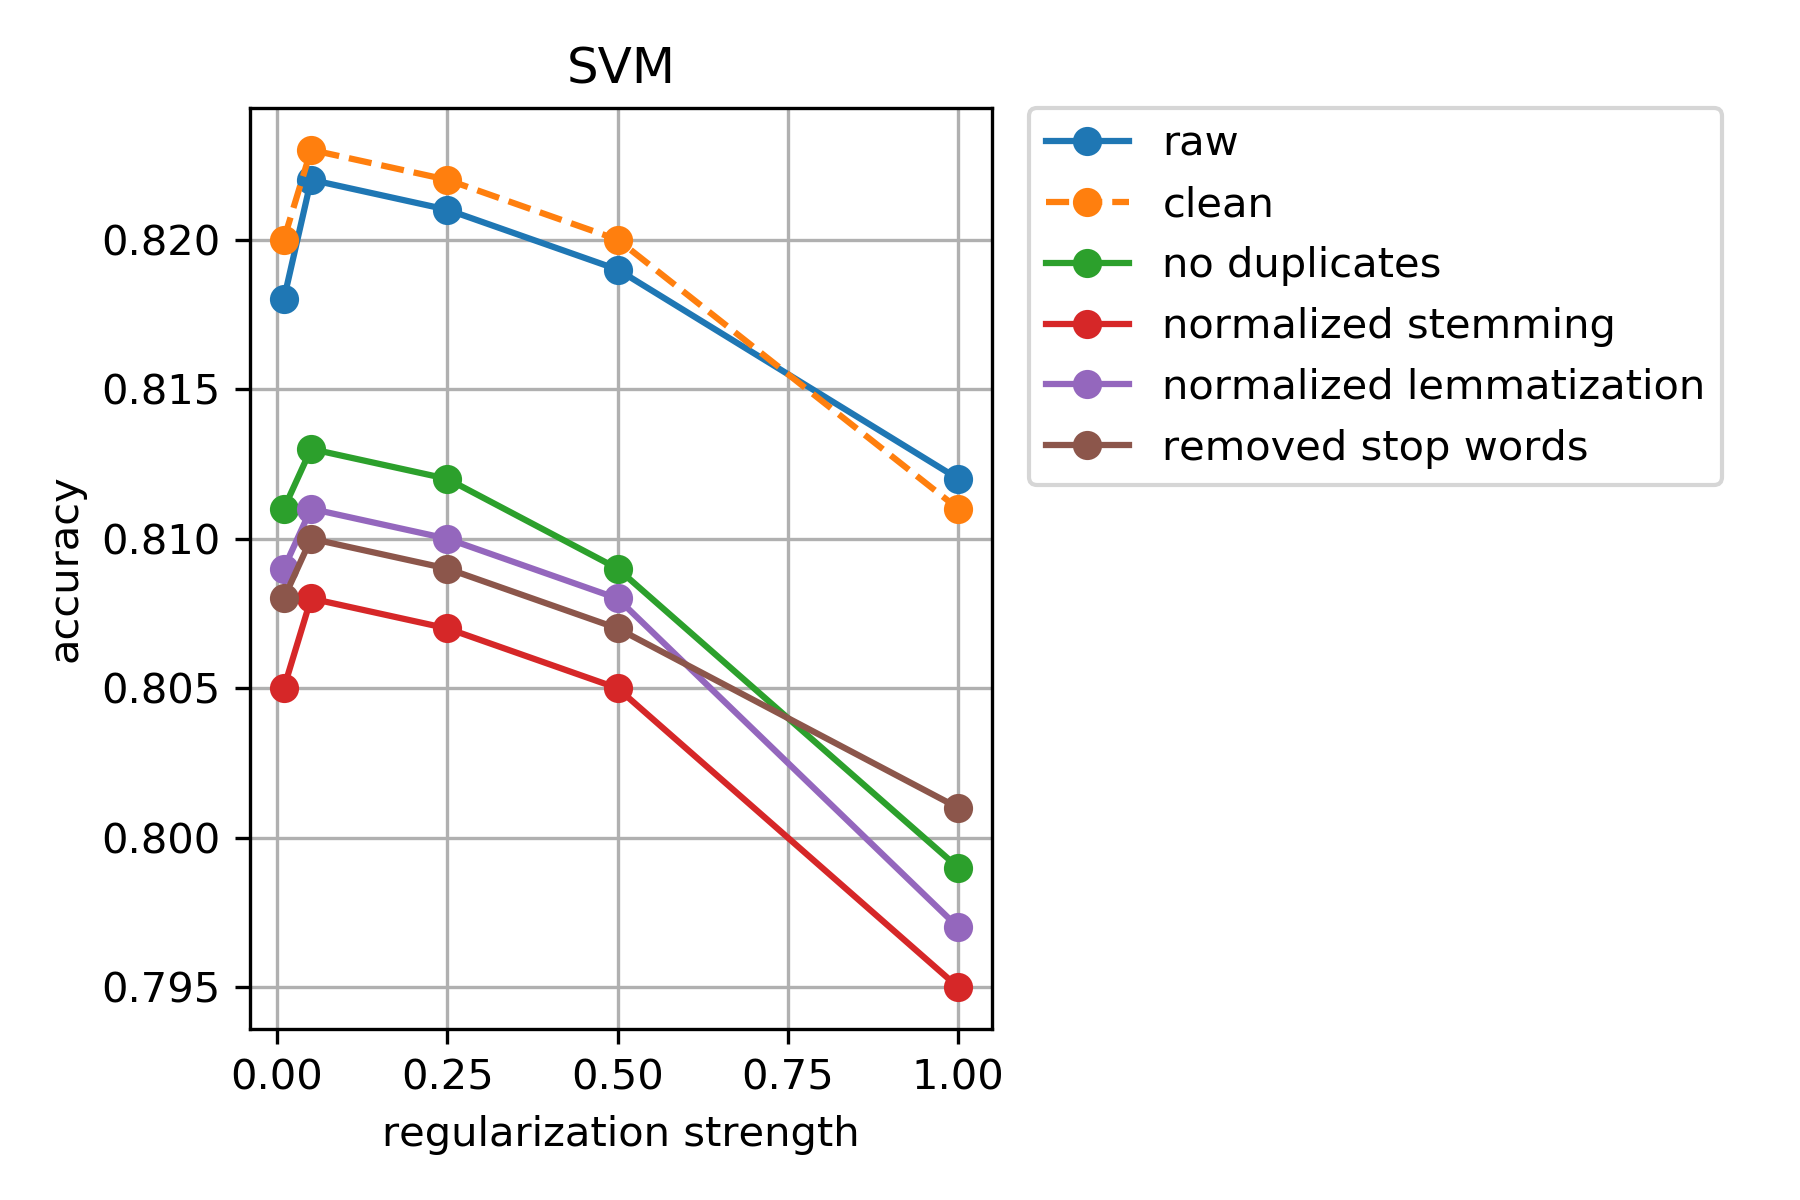
\includegraphics[width=0.5\textwidth]{../plots/svm.png}
\end{figure}

Overall, SVM performs better than logistic regression. Simple cleaning seems to be enough. Since tweets are short sentences, it is hard to normalize tweets without alterating them too much.

\subsection{Optimization of SVM}
Finally, we optimize the SVM model on cleaned data.

\begin{figure}[h]
	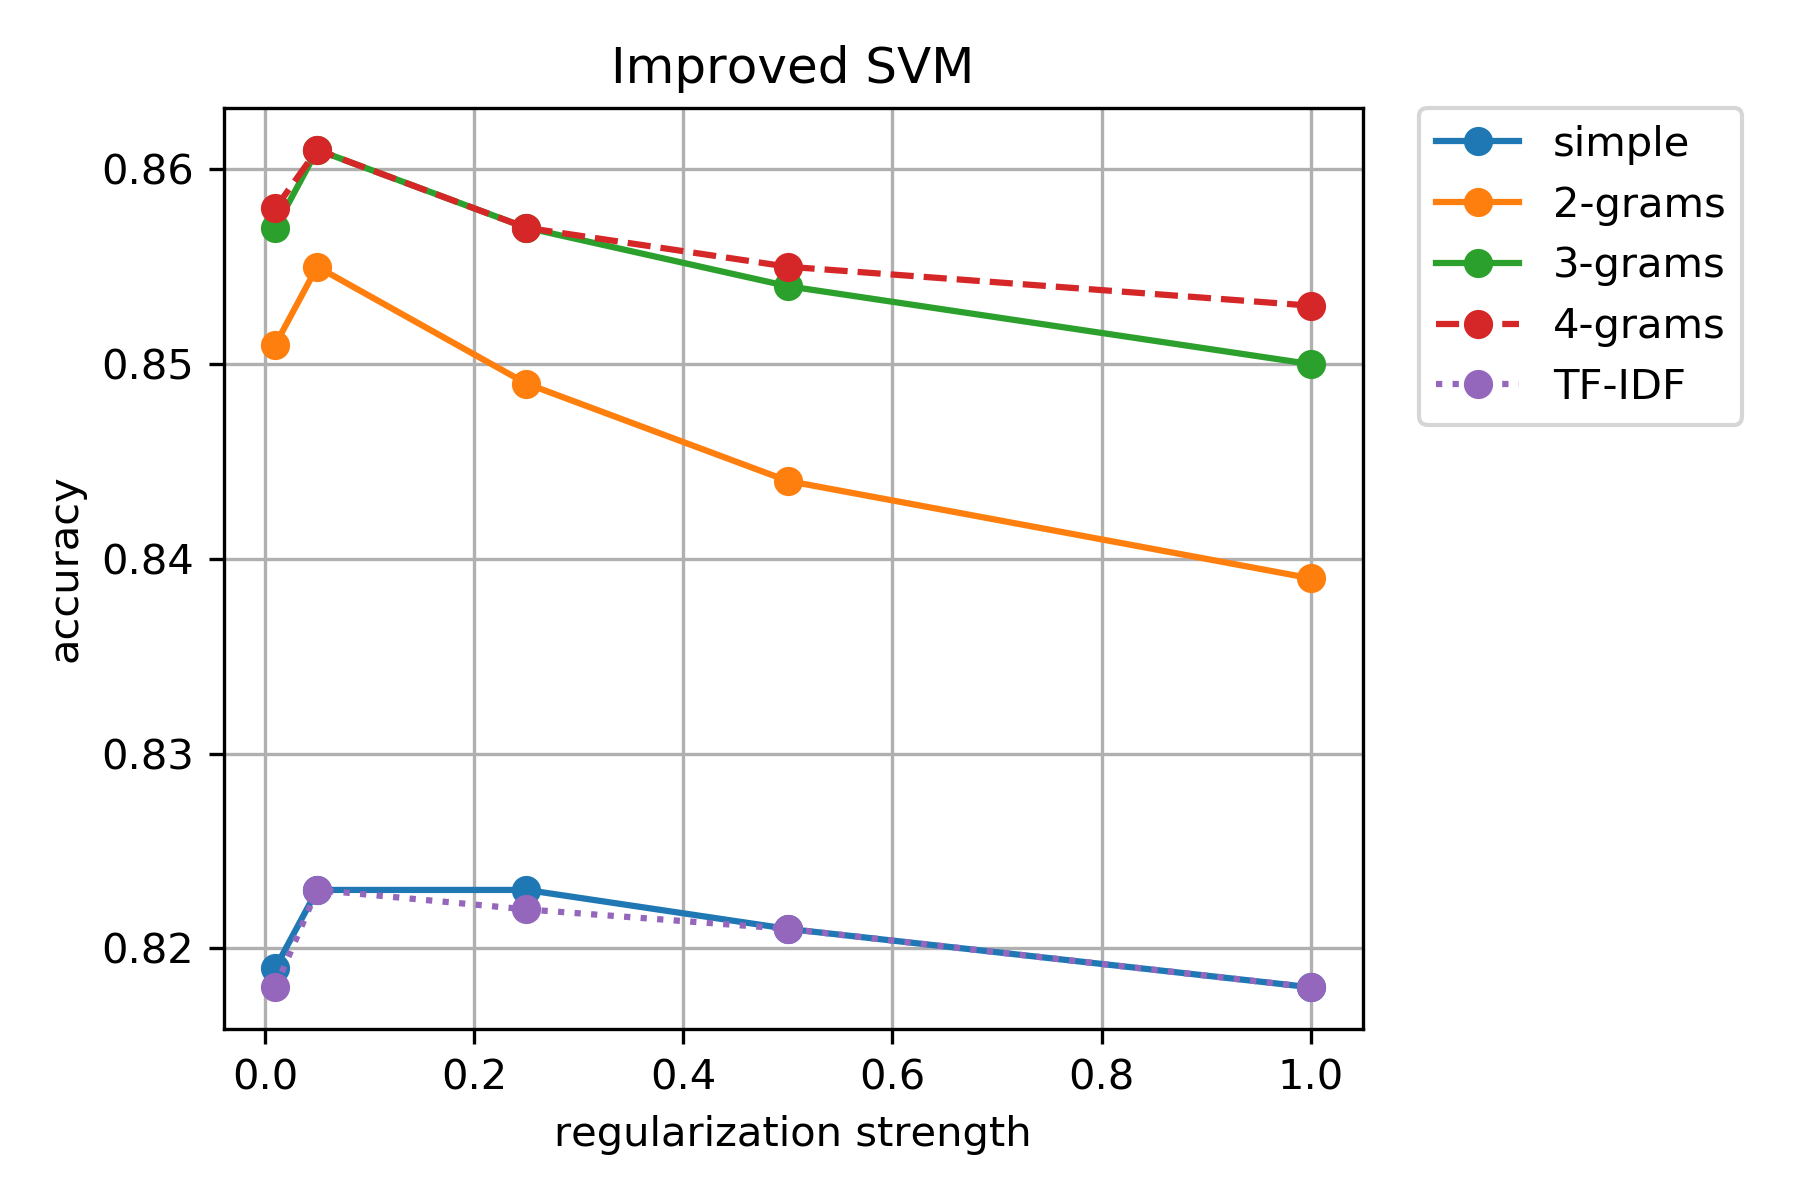
\includegraphics[width=0.5\textwidth]{../plots/improved_svm.png}
\end{figure}

By taking 3 and 4-grams vectorization, we are able to improve from 82\% to 86\% even if 4-grams seems to be the limit before sever overfitting. Nevertheless, this score is confirmed on aicrowd. On the other hand, \textit{TF-IDF} performs similarly to 1-grams as tweets are short and words tend to appear only once in them.

\section{Neural Networks}

\subsection{Preprocessing}
To clean our data, we use an algorithm similar to the one in Kim Yoon's paper\cite{kimyoonpaper} and code\cite{kimyooncode}. We remove duplicates on the training set and separate known contractions: for example, "don't" becomes "do n't".

\subsection{Embedding and Neural Nets}
First, each tweet is transformed into a vector. We implement
GloVE algorithm, the results are not satisfiing (65\%-70\% accuracy). Therefore, we use an embedding with 200 features
provided by the Stanford University which is also based on GloVE algorithm but on a larger Twitter dataset\cite{glovepaper, gloveembedding}. 
Then, we compute the vector for each tweet as the numerical average of each vector corresponding to the 
words of which it is composed.

To do the neural nets and the training, we use the Tensorflow library from Google and run it on Google Colab to benefit from their GPUs.

The NN configurations that give the best results are the one with 
fewer hidden layers but lots of neurons per layer. We also add in some of them dropout layers with $p\in [0.05, 0.2]$ 
depending of the size of the layer before\cite{dropoutkeras}.
The best achieves 84.3\% on aicrowd with one input layer of $200$, one hidden layer of $100,000$, one dropout 
layer with $p=0.15$ and an output layer of 2 nodes. All hidden layers use the ReLU function, other activation functions give poorer results. The output layer uses softmax activation function.

We use standard accuracy as loss function. The optimizer used is first 'Adam' which we replace by SGD for better results.

We try to train the NN on TPUs provided by Google Colab but as everything is in beta, it does not work as expected.

The number of epochs can only be approximated due to all the crashes encountered on Colab but lives around 200 to 250 per model. Around 300 epochs, model starts to overfit and score goes down.

Considering the difficulties encountered during training process due mainly to the computational cost, we keep the ones providing the best scores on aicrowd among all our tries. 
Here is a list of structures and their corresponding score on aicrowd. Only the hidden layers are shown.
\begin{itemize}
  \item \textbf{$81.8\%$}: $\dots \rightarrow 25000\rightarrow 1000\rightarrow 500\rightarrow \dots$
  \item \textbf{$84.2\%$}: $\dots \rightarrow 1000\rightarrow \text{Drop}\rightarrow 1000
  \rightarrow \text{Drop}\rightarrow 1000\rightarrow \text{Drop}\rightarrow 1000
  \rightarrow \text{Drop}\rightarrow 1000\rightarrow \text{Drop}\rightarrow \dots$ where Drop is a dropout layer with $p=0.1$.
  \item \textbf{$84.3\%$}: $\dots \rightarrow 100000\rightarrow \text{Drop}\rightarrow \dots$ where Drop is a dropout layer with $p=0.15$. 
\end{itemize}

\subsection{Convolutional Neural Networks}
We used the following libraries to compare three CNN models and their variations.
\begin{itemize}
	\setlength\itemsep{1px}
	\item Python 3.8
	\item Google Colab
	\item Scikit-learn
	\item Tensorflow
	\item Keras
\end{itemize}

We use the same embedding matrix as for NN\cite{glovepaper, gloveembedding}. To reduce the computational complexity, we cut the embedding matrix to the most used word vectors and tweets. We detect that the maximum number of useful tokens in our data set is 199\label{199}.

We split our datasets into $75\%$ training and $25\%$ validation. Then, we tokenize with Keras and pad the result so that each array has the same length.

\subsubsection{Method 1}
We use a model similar to article\cite{cnn1} with our reduced version of Stanford's embedding and add a dropout layer of 0.2 before the last dense layer to counter overfitting.

\subsubsection{Method 2}
We use the same model as a simplified version\cite{cnn2} of Kim Yoon's paper\cite{kimyoonpaper} with our own embedding.

\subsubsection{Method 3}
We use the same model as proposed in Keras' blog\cite{cnn3} with our own embedding, sigmoid functions for the last layer, adam as optimizer and binary crossentropy for loss.
Since that method works well, we try some variation: add 1 to 3 dropout layers, more units (200 or 1000 instead of 128) in the first dense layer and bigger output dimensions (256 or 512 instead of 128) for the first Conv1D layer. 

\begin{figure}[h]
	\centering
	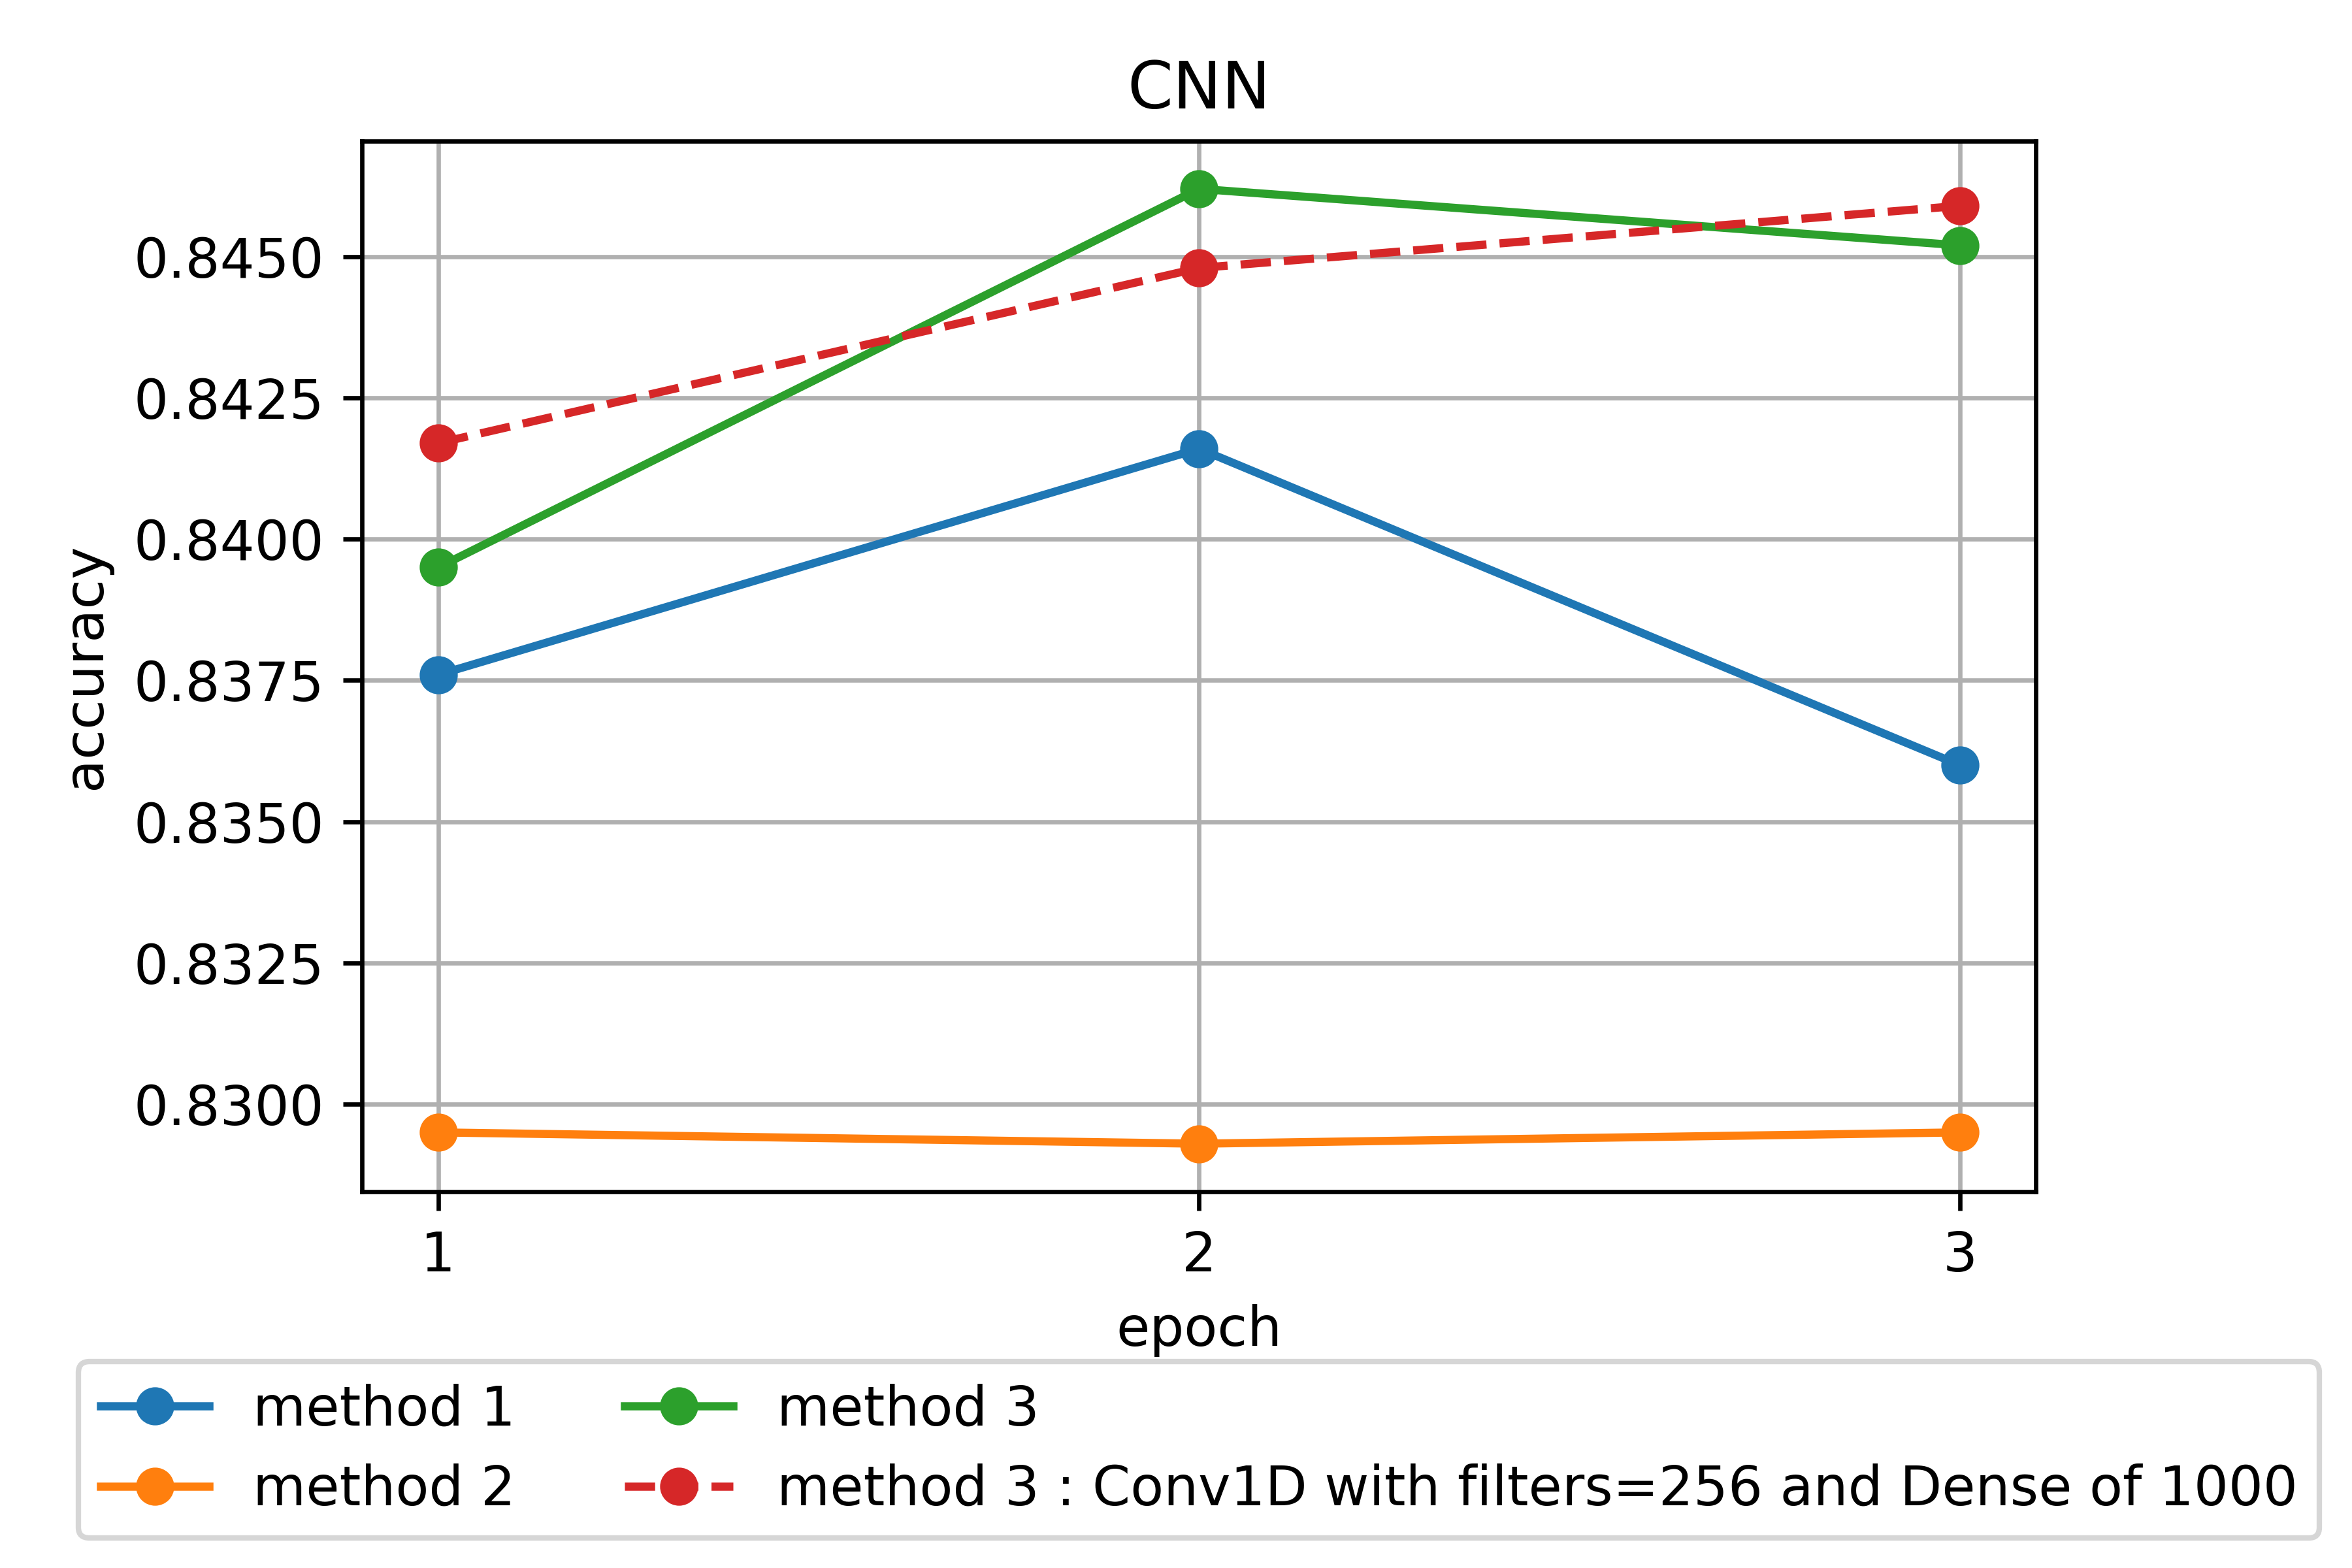
\includegraphics[width=0.5\textwidth]{../plots/cnn.png}
\end{figure}

Overall, the best CNN method is the third one. It obtains a score of $84.9\%$. In CNN figure, the accuracy is computed only for 3 epochs since after the third epoch, every model is overfitting, irrespective of any added dropout.

\section{BERT}
BERT (Bidirectional Encoder Representations from Transformers)\cite{bertpaper} is a training process made at Google. Instead of reading a sentence in a certain order, it uses the entire sequence simultaneously.

We use ktrain library\cite{ktrain} and derive a solution from its tutorial on text classification to use BERT on our datasets. We remove duplicates from our training set and then split it in $75\%$ for training and $25\%$ for validating. To reduce the ressources consumption, we fix the batch size to 10 and the maximal number of tokens to consider to 199, as explained in \ref{199}. Based on the original paper, we use a learning rate of $2*10^{-5}$. We limit it to one epoch with the fit\_onecycle method because it is time consuming. This technique corresponds to our best submission on aicrowd with an accuracy of $87.6\%$ and an F-1 score of $87.9\%$.

We increase the maximal number of tokens to 400, to correspond to the reality of our raw dataset. This decreases our score. Using 3 epochs, a maximal number of tokens of 128 and a batch size of 32 also reduced our accuracy on aicrowd.

\section{Final Discussion}
During this project, we take the opportuinity to experiment multiple machine learning techniques from the most traditional ones up to the newest ones. Moreover, we compared different ideas to preprocess the provided datasets and adapt already tested methods to our project.

Extracting meaningful informations from tweets is a challenging task. They are small pieces of text and users often write concisely and not always in proper English. There are lots of different spellings and variations for a same word and our algorithms struggle to interpret them as one.

To face this difficulty, the dataset could be larger and larger but this would also increase the computational requirements.

The neural networks are powerful tools but the computational power required to train them 
is enormous. This makes them painful to use with our datasets specially on Google Colab which does not let us make long calculation without logging out. 

Given our results, it seems that the logistic regression and the support-vector machine give their best here. We think that we go to the limits of these techniques. 

The newer techniques like BERT perform better but require lots of time and memory. They give better results than techniques cited above but the latter achieves a relatively close 
performance in a smaller amount of time and with less resources. Their computation over accuracy ratio is more reasonable. So they do not become obsolete in our opinion.

In future works, we would like to asses other techniques that look promising like the recurrent neural networks and more precisely the long-short term memory as we still have margin for improvement. These techniques seem to be well suited for text analysis due to their capabilities to remember previous words while they are processing others. As human 
language is based on aligning words together to make sense, it seems natural to process words considering the ones around as well as their structure. 

In the end, teaching a machine to learn from noisy and inconsistent data such as tweets to predict the sentiment expressed by their content is not an easy task.

\clearpage
\onecolumn

\begin{thebibliography}{9}
	\bibitem{kimyoonpaper}
		KIM, Yoon. Convolutional neural networks for sentence classification. arXiv preprint arXiv:1408.5882, 2014.
	\bibitem{kimyooncode}
		CNNs for sentence classification
		\\\url{https://github.com/yoonkim/CNN\_sentence}
	\bibitem{glovepaper}
		PENNINGTON, Jeffrey, SOCHER, Richard, et MANNING, Christopher. Glove: Global vectors for word representation. In : Proceedings of the 2014 conference on empirical methods in natural language processing (EMNLP). 2014. p. 1532-1543.
	\bibitem{gloveembedding}
		GloVE Twitter pre-trained word vectors
		\\\url{https://nlp.stanford.edu/projects/glove}
	\bibitem{bertpaper}
		DEVLIN, Jacob, CHANG, Ming-Wei, LEE, Kenton, et al. Bert: Pre-training of deep bidirectional transformers for language understanding. arXiv preprint arXiv:1810.04805, 2018.
	\bibitem{bertcode}
		BERT Text Classification in 3 Lines of Code Using Keras
		\\\url{https://towardsdatascience.com/bert-text-classification-in-3-lines-of-code-using-}
		\\url{-keras-264db7e7a358}
	\bibitem{ktrain}
		Ktrain library
		\\\url{https://github.com/amaiya/ktrain}
	\bibitem{cnn1}
		How to implement CNN for NLP tasks like Sentence Classification
		\\\url{https://medium.com/saarthi-ai/sentence-classification-using-convolutional-neural-networks-ddad72c7048c}
	\bibitem{cnn2}
		Text Classification by Convolutional Neural Network in Keras
		\\\url{https://github.com/bhaveshoswal/CNN-text-classification-keras}
	\bibitem{cnn3}
		Using pre-trained word embeddings in a Keras model
		\\\url{https://blog.keras.io/using-pre-trained-word-embeddings-in-a-keras-model.html}
	\bibitem{sentianal}
		Sentiment Analysis with Python
		\\\url{https://towardsdatascience.com/sentiment-analysis-with-python-part-1-5ce197074184}
		\\\url{https://towardsdatascience.com/sentiment-analysis-with-python-part-2-4f71e7bde59a}
	\bibitem{stemlema}	
		Stemming and Lemmatization
		\\\url{https://nlp.stanford.edu/IR-book/html/htmledition/stemming-and-lemmatization-1.html}
	\bibitem{dropoutkeras}
	Dropout in (Deep) Machine learning
	\\\url{https://medium.com/@amarbudhiraja/https-medium-com-amarbudhiraja-learning-less-to-learn-better-dropout-in-deep-machine-learning-74334da4bfc5}
\end{thebibliography}

\end{document}
